\section{UUID}
\label{sec:uuid}

Universally Unique Identifiers (UUIDs) sind 128 Bit lange Zeichenfolgen bestehend aus 32 Base-16 encodierten Zeichen. Diese Länge ist ausreichend, sodass zwei zufällig generierte UUIDs mit annähernder Sicherheit nicht identisch sind. Da von den 128 Bits einer UUID 122 Bits zufällig gewählt werden, kann die Wahrscheinlichkeit für eine Überschneidung zweier zufällig generierter UUIDs mittels der Abschätzung $p(n) \approx 1 - e^{-n^2 / (2 \cdot 2^{122})}$ approximiert werden. Eine Überschneidung bei der Generierung von einer Milliarde UUIDs tritt also beispielsweise mit einer Wahrscheinlichkeit von weniger als $1 \cdot 10^{-17}$ \% auf. Diese Berechnung setzt allerdings voraus, dass die UUIDs völlig zufällig und mit ausreichender Entropie generiert wurden.

Es gibt aktuell fünf Versionen von UUIDs, wobei die wesentlichen Unterschiede darin bestehen, wie die UUID generiert wird und dadurch wiederum verschiedene Vor- und Nachteile haben. Grafik \ref{fig:UUIDv1} zeigt als ein Beispiel eine UUID der Version 1 und kennzeichnet dessen unterschiedliche Bestandteile mit den dazugehörigen Komponenten-Namen. Die Komponenten \verb|time_low|, \verb|time_mid| und \verb|time_hi_and_version| sind dabei etwa vom aktuellen Zeitpunkt abhängig, während die letzte Komponente von der MAC-Adresse (Media Access Control Adresse) des Gerätes kommt [\cite{uuid}].
%
\begin{figure}[htbp]
	\centering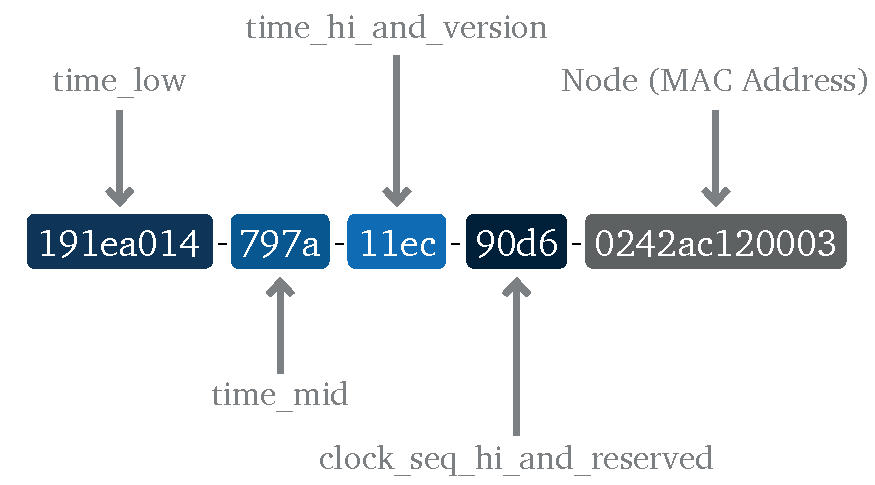
\includegraphics[width=0.7\textwidth]{images/03/UUID.pdf}
    \caption{UUID Version 1 Komponenten}
    \label{fig:UUIDv1}
\end{figure}

Alle Versionen werden aktuell noch für unterschiedliche Anwendungsfälle genutzt. In Tabelle \ref{tab:UUIDversions} werden die Attribute, Stärken und Schwächen der verschiedenen Versionen verglichen.
%
\WarningsOff[paralist]
\bgroup
\def\arraystretch{1.5}
\vspace{5mm}\begin{table}[htbp]
    \centering
    \begin{tabularx}{155.8mm}{@{}>{\bfseries}p{10mm}@{\hspace{0.0em}}X@{\hspace{0.8em}}X@{\hspace{0.8em}}X@{}}
        \rowcolor{dikblue} \mbox{\color{white}\textbf{Ver.}} & \mbox{\color{white}\textbf{Attribute}} & \mbox{\color{white}\textbf{Stärken}} & \mbox{\color{white}\textbf{Schwächen}} \\
        \begin{compactenum}[] \item \hspace{-2.0mm}1 \end{compactenum} & \begin{compactenum}[•] \item Zeitstempel abgeleitet von der internen Uhr des Geräts \item \texttt{Node} ist einzigartig für das Erzeugungsgerät \end{compactenum} & \begin{compactenum}[•] \item Einzigartigkeit: Eine Überschneidung ist aufgrund von Geräte- und zeitbezogene Informationen praktisch unmöglich \end{compactenum} & \begin{compactenum}[•] \item Anonymität: MAC-Adresse und Zeitstempel verraten Uhrzeit und Gerät der Generierung \end{compactenum} \\ \hline
        \begin{compactenum}[] \item \hspace{-2.0mm}2 \end{compactenum} & \begin{compactenum}[•] \item Zusätzliche Kennnummer wird Generierung einbezogen \end{compactenum} & \begin{compactenum}[] \item \hspace{0.5mm}\textit{Identisch zu Version 1} \end{compactenum} & \begin{compactenum}[] \item \hspace{0.5mm}\textit{Identisch zu Version 1} \end{compactenum} \\ \hline
        \begin{compactenum}[] \item \hspace{-2.0mm}3 \end{compactenum} & \begin{compactenum}[•] \item Verwendet einen Hashing-Algorithmus, um eine zufällige Zeichenfolge basierend auf dem Namespace zu generieren, in dem die UUID generiert wurde. \item Keine Geräte- oder Zeitkomponenten \end{compactenum} & \begin{compactenum}[•] \item Anonymität: Gehashte Namespace-Identifikatoren verbergen den Ursprung der UUID \item Reproduzierbarkeit: Mit den gleichen Eingaben kann eine gleich UUID generiert werden \end{compactenum} & \begin{compactenum}[•] \item Einzigartigkeit: Verlässt sich auf einen vom Benutzer eingegebenen Namen, um zufällige Komponente zu generieren \item Reproduzierbarkeit: Mit den gleichen Eingaben kann eine gleich UUID generiert werden \end{compactenum} \\ \hline
        \begin{compactenum}[] \item \hspace{-2.0mm}4 \end{compactenum} & \begin{compactenum}[•] \item Zufällig generiert ohne zeit-, geräte- oder umfeldbezogene Komponenten \end{compactenum} & \begin{compactenum}[•] \item Am zufälligsten \item Keine Möglichkeit Herkunft zu bestimmen \end{compactenum} & \begin{compactenum}[•] \item Keine Möglichkeit Herkunft zu bestimmen \end{compactenum} \\ \hline
        \begin{compactenum}[] \item \hspace{-2.0mm}5 \end{compactenum} & \begin{compactenum}[•] \item Ähnlich zu Version 3, jedoch mit einem sichereren Hashing-Algorithmus \end{compactenum} & \begin{compactenum}[] \item \hspace{0.5mm}\textit{Identisch zu Version 3} \end{compactenum} & \begin{compactenum}[] \item \hspace{0.5mm}\textit{Identisch zu Version 3} \end{compactenum} \\
    \end{tabularx}
    \caption{Vergleich der UUID Versionen [\cite{uuidVersions}]}
    \label{tab:UUIDversions}
\end{table}
\egroup
\WarningsOn[paralist]
